%%%%%%%%%%%%%%%%%%%% author.tex %%%%%%%%%%%%%%%%%%%%%%%%%%%%%%%%%%%
%
% sample root file for your "contribution" to a contributed volume
%
% Use this file as a template for your own input.
%
%%%%%%%%%%%%%%%% Springer %%%%%%%%%%%%%%%%%%%%%%%%%%%%%%%%%%


% RECOMMENDED %%%%%%%%%%%%%%%%%%%%%%%%%%%%%%%%%%%%%%%%%%%%%%%%%%%
\documentclass{svmult}

% choose options for [] as required from the list
% in the Reference Guide

\usepackage{type1cm}        % activate if the above 3 fonts are
                            % not available on your system
%
\usepackage{makeidx}         % allows index generation
\usepackage{graphicx}        % standard LaTeX graphics tool
                             % when including figure files
\usepackage{multicol}        % used for the two-column index
\usepackage[bottom]{footmisc}% places footnotes at page bottom
\usepackage{multirow}

\usepackage{newtxtext}       % 
\usepackage{newtxmath}       % selects Times Roman as basic font

\usepackage{amsmath}
% see the list of further useful packages
% in the Reference Guide

\makeindex             % used for the subject index
                       % please use the style svind.ist with
                       % your makeindex program

%%%%%%%%%%%%%%%%%%%%%%%%%%%%%%%%%%%%%%%%%%%%%%%%%%%%%%%%%%%%%%%%%%%%%%%%%%%%%%%%%%%%%%%%%

\begin{document}

\title*{Cooking Activity Recognition with Convolutional LSTM using Multi-label Loss Function and Majority Vote}
\titlerunning{Cooking Activity Recognition with Convolutional LSTM}
% Use \titlerunning{Short Title} for an abbreviated version of
% your contribution title if the original one is too long
\author{Atsuhiro Fujii, Daiki Kajiwara, Kazuya Murao}
% Use \authorrunning{Short Title} for an abbreviated version of
% your contribution title if the original one is too long
\institute{Asuhiro Fujii \at Graduate School of Information Science and Engineering, Ritsumeikan University, 1-1-1 Nojihigashi, Kusatsu, Shiga 525-8577, Japan %\email{atsuhiro.fujii@iis.ise.ritsumei.ac.jp}
\and Daiki Kajiwara \at Graduate School of Information Science and Engineering, Ritsumeikan University, 1-1-1 Nojihigashi, Kusatsu, Shiga 525-8577, Japan %\email{daiki.kajiwara@iis.ise.ritsumei.ac.jp}
\and Kazuya Murao \at Graduate School of Information Science and Engineering, Ritsumeikan University, 1-1-1 Nojihigashi, Kusatsu, Shiga 525-8577, Japan \email{murao@cs.ritsumei.ac.jp}}
%
% Use the package "url.sty" to avoid
% problems with special characters
% used in your e-mail or web address
%
\maketitle

\abstract*{Each chapter should be preceded by an abstract (no more than 200 words) that summarizes the content. The abstract will appear \textit{online} at \url{www.SpringerLink.com} and be available with unrestricted access. This allows unregistered users to read the abstract as a teaser for the complete chapter.
Please use the 'starred' version of the \texttt{abstract} command for typesetting the text of the online abstracts (cf. source file of this chapter template \texttt{abstract}) and include them with the source files of your manuscript. Use the plain \texttt{abstract} command if the abstract is also to appear in the printed version of the book.}

\abstract{This paper reports the Cooking Activity Recognition Challenge by team Rit's cooking held in the International Conference on Activity and Behavior Computing (ABC 2020).
Our approach leverages convolution layer and LSTM to recognize macro activities (recipe), and micro activities (body motion). For micro activity consisting of multiple labels in a segment, loss is calculated using BCEWithLogistsLoss function in PyTorch for each body part, and then the final decision is made by majority vote by the body parts.
%We have trained the model using the training data provided and achieved ***\% accuracy for recipe and ***\% F1 score for body motions.
}

\section{Introduction}
\label{sec:intro}
This paper reports the solution of our team ``Rits's cooking'' to Cooking Activity Recognition Challenge held at International Conference on Activity and Behavior Computing (ABC2020).

As one of the methods for human activity recognition with neural network, Ordóñez et al. proposed deep convolutional and LSTM reccurent neural network\cite{deepconv}. Most conventional methods consider single-label activities which means only one non-overlapping label is given to the input data. However, the cooking activity dataset we handle in this challenge includes micro and macro activity. The micro activity consists of a set of single segment with multiple labels. In addition, the number of samples in a segment for each sensor are different.

In this paper we constructed a network with convolutional layer and LSTM layer for sensors at each body part. Hand crafted features are employed as an input of the network. For micro activities, BCEWithLogistsLoss is used as loss function to evaluate multi-label data. Four decisions obtained with the networks are the merged to one final output by majority vote.

This paper is organized as follows: Section 2 introduces the challenge, section 3 explain our model, section 4 evaluates our model, and section 5 conclude this paper.

\section{Challenge}
\label{sec:challenge}
In this challenge, each team competes with each other on the recognition accuracy of cooking activities. This section introduces the challenge goal, the dataset, and the evaluation criteria.

\subsection{Challenge Goal}
The goal of the Cooking Activity Recognition Challenge is to recognize both the macro activity (recipe) and the micro activities took place in a 30-second window based on acceleration data and motion capture data.

The training dataset contains data about 3 subjects and contains all activity labels. The test dataset contains data about the other subject and is not labeled. Participants must submit their predicted macro and micro activities on the test dataset using their models.

\subsection{Dataset}
\label{sec:dataset}
\subsubsection{Sensors and subjects}
The data has been collected from four subjects who had attached two smartphones on the right arm and left hip, two smartwatches on both wrists, and one motion capture system with 29 markers. The subjects cooked three recipes (sandwich, fruit salad, cereal) five times each by following a script for each recipe, but acted as naturally as possible.

\subsubsection{Data structure}
Training data contains data from three subjects (subject 1, 2, 3) out of the four subjects and test data contains the data from the fourth subject (subject 4).

Each recording has been segmented into 30-second segments. Each segment was assigned a random identifier, so the order of the segments is unknown. Each sensor data segment is stored in a separate file with the segment-id used to identify related files. Segments of the four sensors at same time frame were assigned same identifier. 

Groundtruth for all the segments are stored in one file. This file contains one row per file, and each row contains the file name, the macro activity and the micro activities all separated by commas; e.g., {\tt [subject1\verb|_|file\verb|_|939,fruitsalad,Take,Peel,]}, which means that in segment 939 the subject 1 took something and peel something while making fruit salad. The micro activity is multi-label recognition task.

The macro activity is three classes: sandwich, fruitsalad, and cereal and the micro activity is ten classes: Cut, Peel, Open, Take, Put, Pour, Wash, Add, Mix, other.

\subsubsection{Statistics}
Table \ref{tab:stats} shows the number of segments for each subject, the number of annotated classes of macro activity (one in this challenge), max, mean, and min number of annotated classes of micro activities, max, mean, and min length of the segments.

\begin{table}[h]
    \centering
    \caption{Statistics of the dataset.}
    \begin{tabular}{c|l|c|c|c|c|c|c|c|c}\hline\hline
        Subject &Body part& \# of segments &\# of macro& \multicolumn{3}{c|}{\# of micro}& \multicolumn{3}{c}{Length}  \\
         &&&&max&mean&min&max&mean&min\\\hline
        \multirow{4}{*}{1} & left hip& \multirow{4}{*}{80} &\multirow{4}{*}{1}&\multirow{4}{*}{5}&\multirow{4}{*}{2.09}&\multirow{4}{*}{1}  &159&131.9&1 \\
          & left wrist&&&&&&8191&2945&0\\
          & right arm&&&&&&1470&1309&8\\
          & right wrist&&&&&&8257&4484&0\\\hline
        \multirow{4}{*}{2}& left hip& \multirow{4}{*}{105}&\multirow{4}{*}{1}&\multirow{4}{*}{6}&\multirow{4}{*}{2.26}&\multirow{4}{*}{1}&505&428.3&10   \\
          & left wrist&&&&&&5986&2171&0\\
          & right arm&&&&&&1500&1272&8\\
          & right wrist&&&&&&2992&2465&0\\\hline
        \multirow{4}{*}{3} & left hip& \multirow{4}{*}{103}&\multirow{4}{*}{1}&\multirow{4}{*}{6}&\multirow{4}{*}{2.30}&\multirow{4}{*}{1}&519&429.3&32  \\
          & left wrist&&&&&&5529&774.6&0\\
          & right arm&&&&&&1594&1182&164\\
          & right wrist&&&&&&5938&3559&0\\\hline
        \multirow{4}{*}{4} & left hip & \multirow{4}{*}{180}&\multirow{4}{*}{1}&\multirow{4}{*}{Unknown}&\multirow{4}{*}{Unknown}&\multirow{4}{*}{Unknown}&534&406.7&46 \\
          & left wrist&&&&&&7143&1126&0\\
          & right arm&&&&&&1479&1233&86\\
          & right wrist&&&&&&8761&2080&0\\\hline
    \end{tabular}
    \label{tab:stats}
\end{table}

\subsection{Evaluation criteria}
Submissions will be evaluated by the average of the accuracy of macro activity classification (ma) and the average accuracy of micro-activity classification (mi). That is (ma+mi)/2.

The average accuracy of micro-activity classification is based on the multi-label accuracy formula. The accuracy of one sample is given by the following equation; the number of correct labels predicted (logical product of prediction set $P$ and groundtruth set $G$) divided by the number of total true and predicted labels (logical sum of $P$ and $G$).

\begin{equation}\label{eqn:accuracy}
    accuracy = \frac{P\cap G}{P\cup G}
\end{equation}

\section{Method}
\label{sec:method}
This section describes the preprocessing to obtain the features from the raw data, the structure of the model, the loss function and the optimizer, and the process of obtaining the activity labels from the predictions obtained by the one-hot vector. Note that our method does not use motion capture data.

%This section explains our method that recognizes macro and micro activities from acceleration data for each segment. Note that our method does not use motion capture data.

%3.3(3.2)に移動しました.
% \subsection{Overview}
% Figure \ref{fig:model} shows the structure of our model. The detailed process in each layer is explained in the later subsections. 
% \begin{figure}[h]
% \sidecaption[t]
% 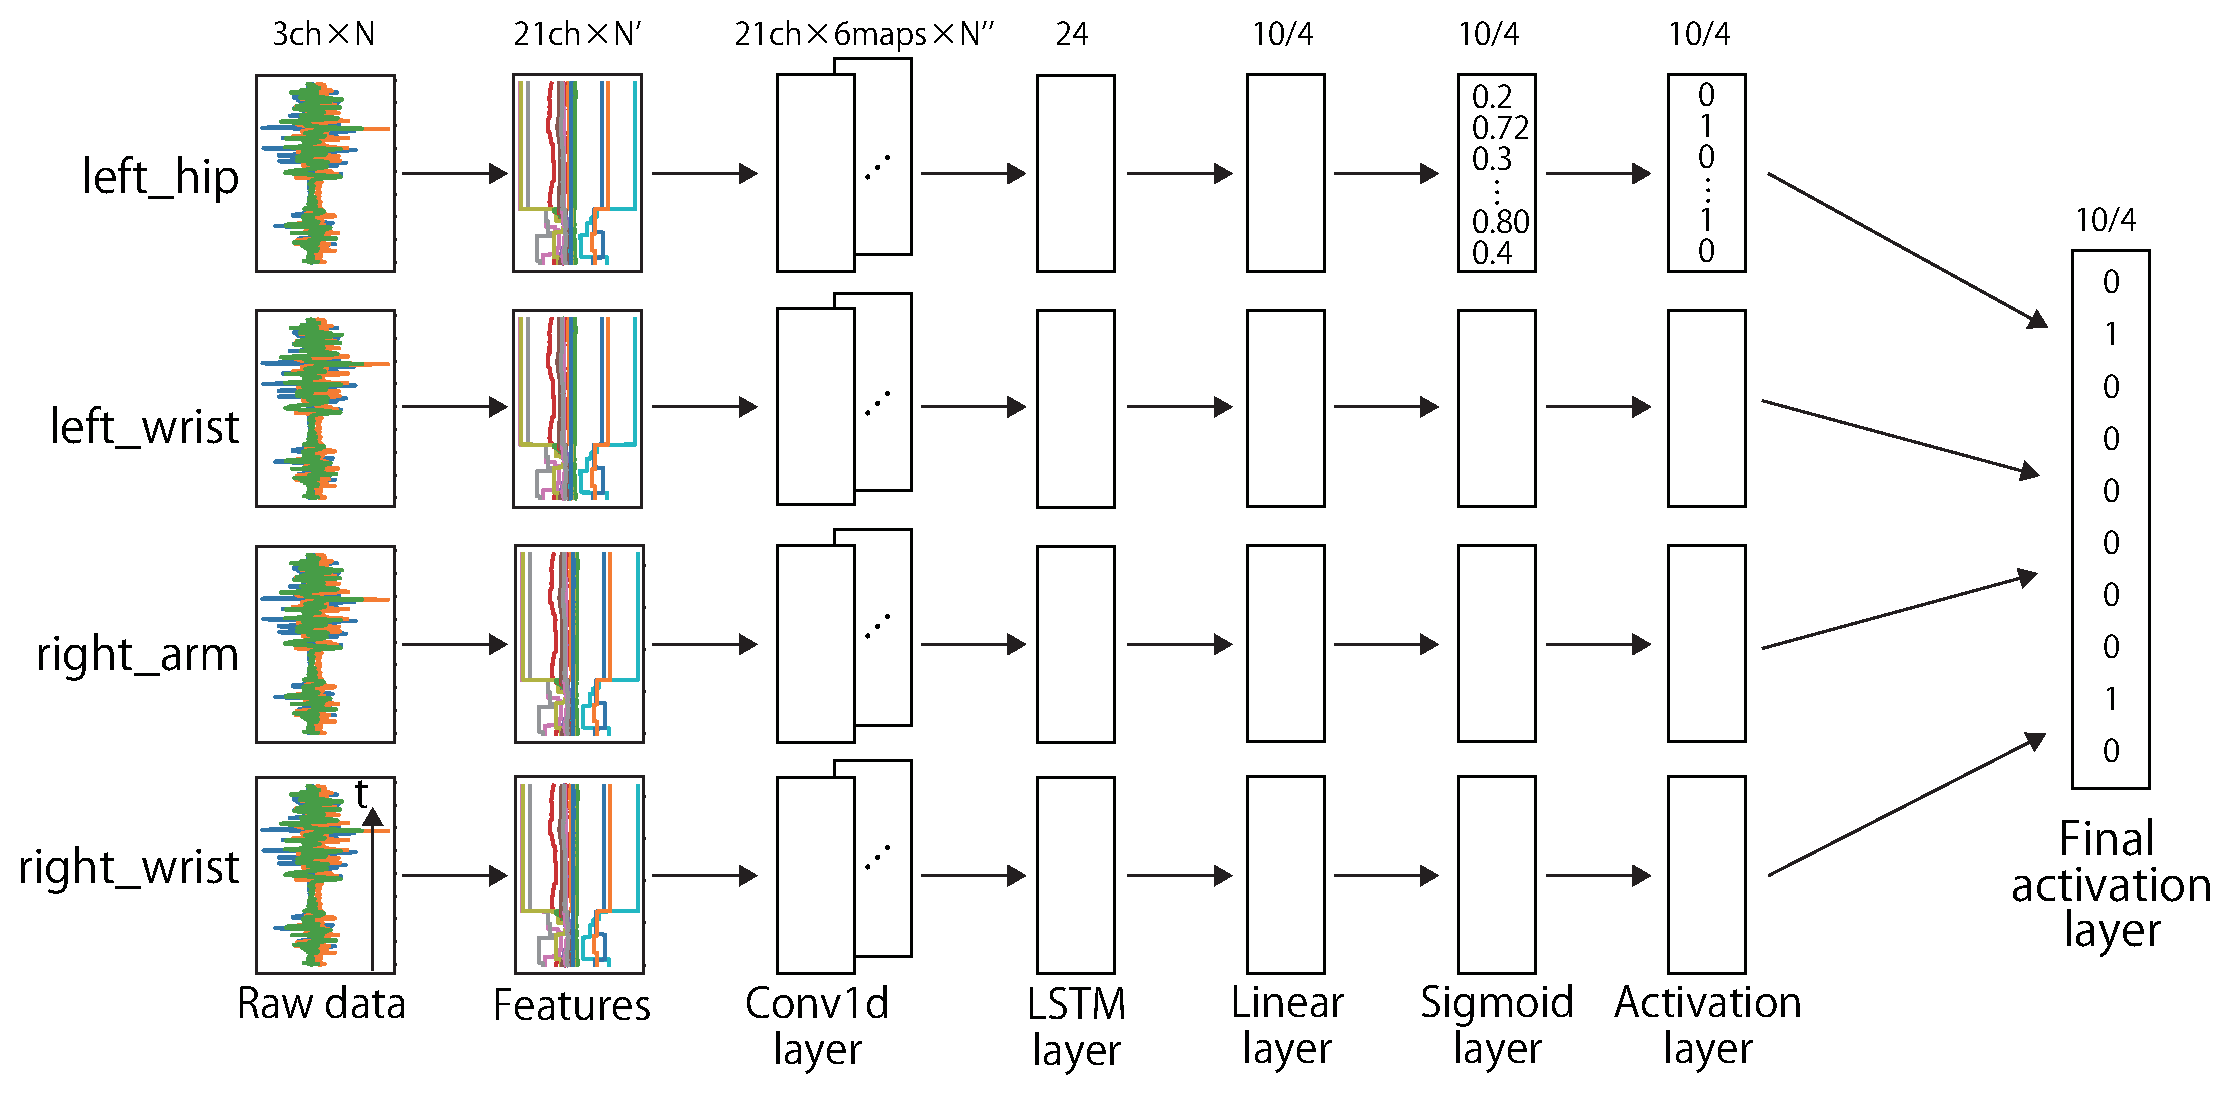
\includegraphics[width=1\linewidth]{Figure_1}
% \caption{Our mode. The first layer is raw data provided as it is. The second layer is hand crafted features consisting of 21 channels. Conv1d layer is one dimensional convolutional layer consisting of 6 maps for 21 channels, 126 maps in total. The 126-channel time-series data will be fed into the next LSTM layer consisting of 24 hidden layer. Then 24 dimensional tensor is shrunk to 10 dimensional tensor, then sigmoid function is applied, one-hot encoded with predetermined threshold. At last, four one-hot encoded vectors are merged and final multi-label prediction is obtained.}
% \label{fig:model}
% \end{figure}

\subsection{Preprocessing}
Hand crafted feature values are extracted from the raw data $[[x_1,\dots, x_N], [y_1, \dots, y_N],$ $[z_1, \dots, z_N]]$, where $x$, $y$, $z$ are raw data of x, y, z axis, and $N$ is the number of samples in a 30-second segment. The features are mean, variance, max, min, root mean square (RMS), interquartile range (IQR), and zero crossing rate (ZCR) for x, y, and z axis, respectively. These features are calculated over a 50ms-window slid in steps of 3 seconds. From the preprocessing, 7 features $\times$ 3 axes = 21 dimensions feature time series are obtained for one sensor. The dataset includes the data obtained at four body parts, therefore this process is conducted for each sensor.

\subsection{Model}
Figure \ref{fig:model} shows the structure of our model.The 21-dimensional feature time-series data is fed into our model consisting of 1d convolutional layer, LSTM layer, linear layer, and Sigmold layer. The process at each layer is as follows:

\begin{figure}[h]
\sidecaption[t]
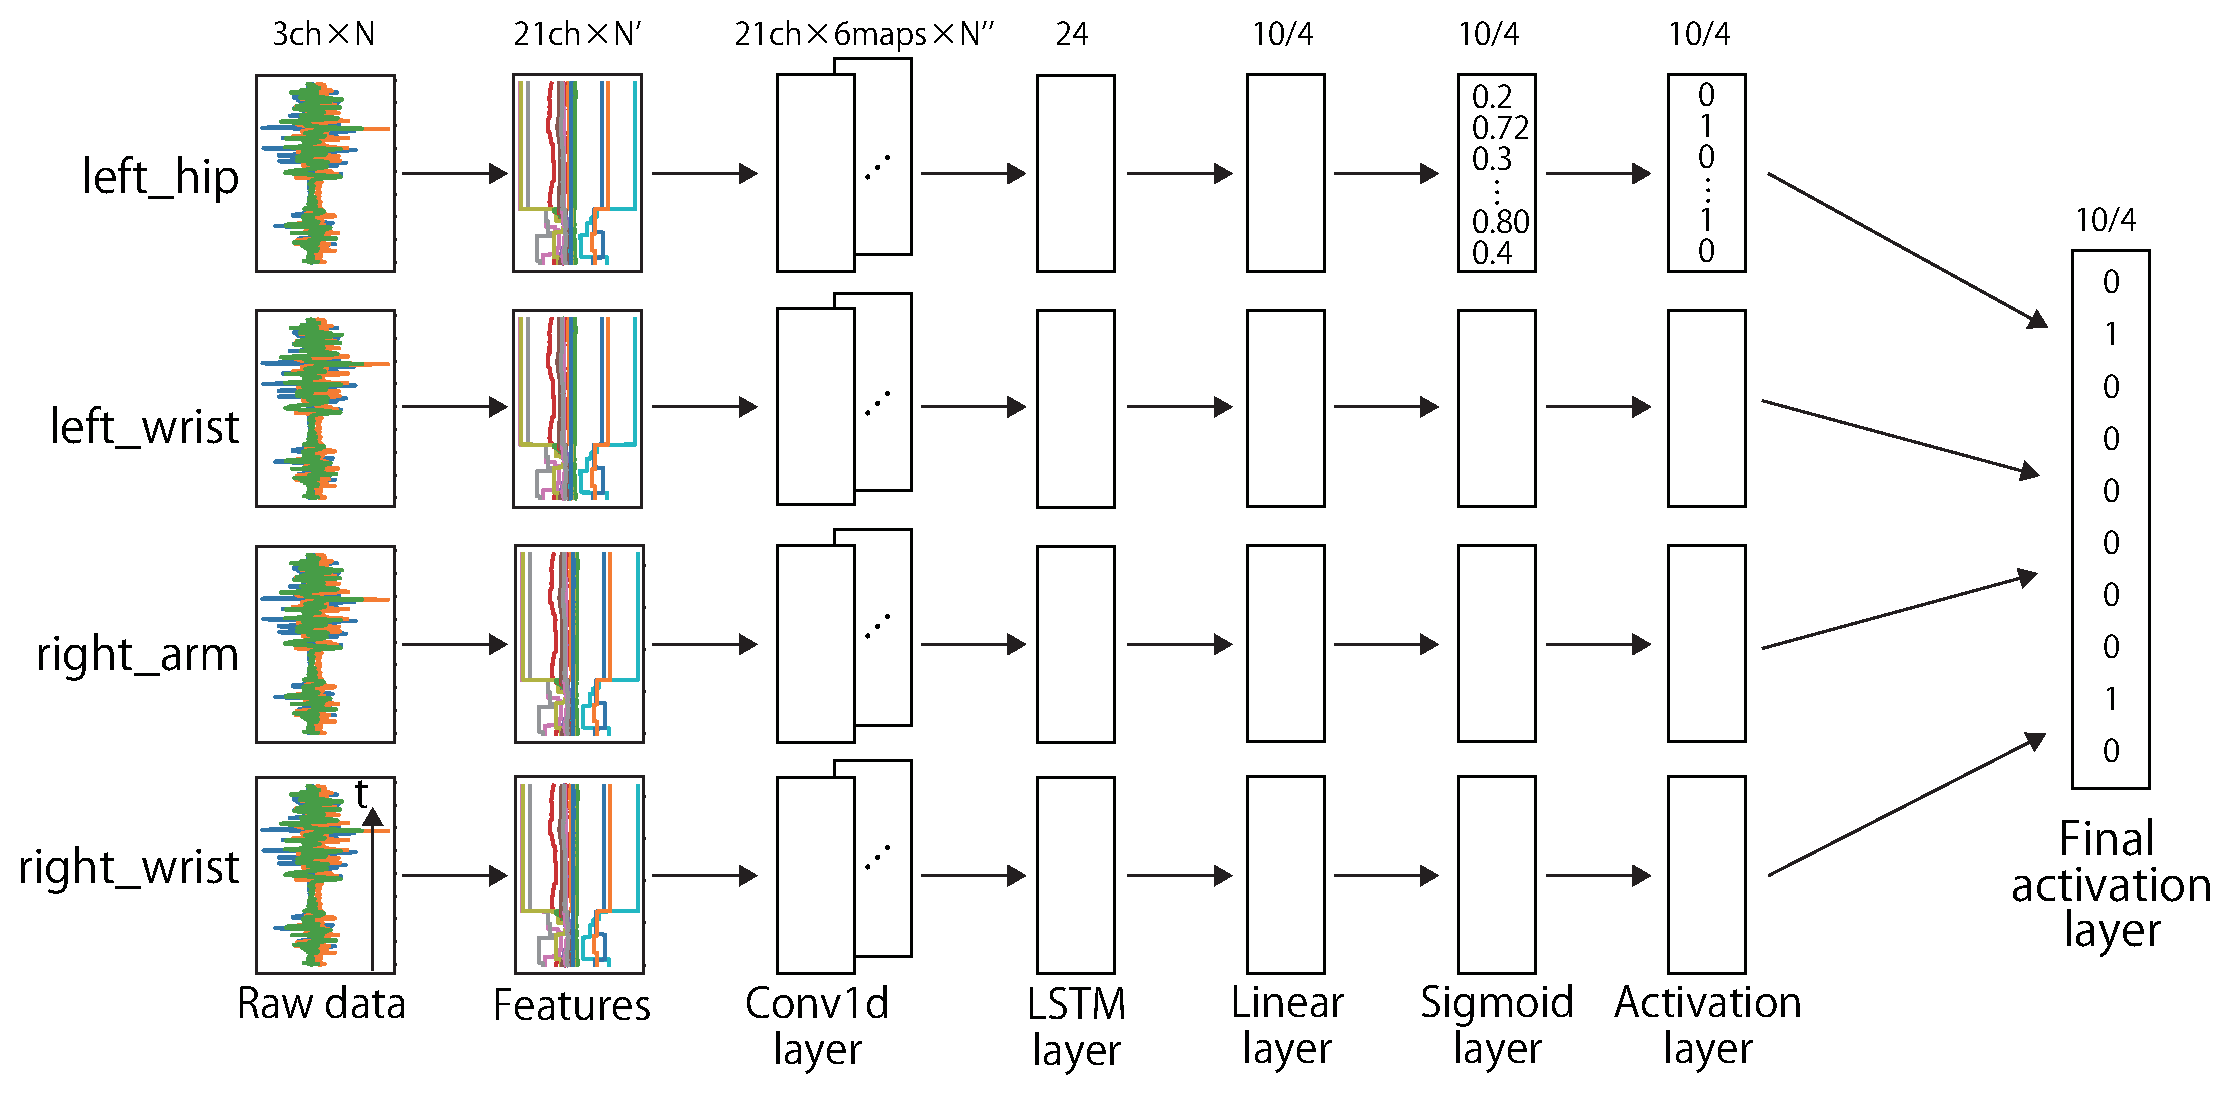
\includegraphics[width=1\linewidth]{Figure_1}
\caption{Our mode. The first layer is raw data provided as it is. The second layer is hand crafted features consisting of 21 channels. Conv1d layer is one dimensional convolutional layer consisting of 6 maps for 21 channels, 126 maps in total. The 126-channel time-series data will be fed into the next LSTM layer consisting of 24 hidden layer. Then 24 dimensional tensor is shrunk to 10 dimensional tensor, then sigmoid function is applied, one-hot encoded with predetermined threshold. At last, four one-hot encoded vectors are merged and final multi-label prediction is obtained.}
\label{fig:model}
\end{figure}

\begin{itemize}
    \item {\bf 1d convolutional layer} has an input of sequence length $N'$ $\times$ 21 channels and an output of sequence length $N''$ $\times$ map size $M$. $N'$ is the length of time-series after the feature extraction, which is smaller than the original raw data. $N''$ is the length of time-series after the convolution, which is $N'-K+1$, where $K$ is the kernel size. $N'$ and $N''$ are variable length because the dataset has deficit values and sampling frequency is different to the sensors. Segments whose length is less than 10 is discarded and not fed in to the model. Kernel size $K$ is set to 10. Map size $M$ is the number of filters and set to $6 \times 21 =126$. Here, the convolution is depthwise, i.e., the convolution is conducted for each channel and there are 6 filters for each channel.  
    
    \item {\bf LSTM layer} has an input of sequence length $\times$ 126 channels and an output of 24 dimensional tensors. The LSTM is many to one. The number of hidden layer is 24 and the last output of the LSTM layers are obtained. At this moment, the output is no longer time-series, but one tensor.
    
    \item {\bf Linear layer} has an input of 24 dimensional flattened tensor and an output of 10/4 dimensional tensors. For macro (recipe) recognition, output is 4 dimensions, for micro activities, output is 10 dimensions.
    
    \item {\bf Sigmoid layer} applies the sigmoid activation function to the 10/4 dimensional tensors, which represents the likelihood of the classes.
    
    \item {\bf Activation layer} has an 10/4 dimensional tensor and an output of 10/4 dimensional one-hot vector. This layer activates the prediction classes whose values are more than the threshold $Th$. For micro activity recognition, the output one-hot vector has multiple 1 elements since the data is multi-labeled, e.g., [0,1,0,0,0,0,0,0,0,0] or [0,0,1,0,1,0,0,0,0,0]. The threshold $Th$ is determined in the training phase by finding the best accuracy by changing the threshold from 0 to 1. For recipe recognition, the vectors in the sigmoid layer are used, not one-hot encoded. 
\end{itemize}



\subsection{Loss Function and Optimizer}
The models for four sensors are trained separately. The model is trained on BCEWithLogistsLoss in PyTorch for micro activities and its weight was set to one for all classes. For macro activity, CrossEntropyLoss in PyTorch is used as loss function. Adam was used for optimizer for macro and micro activities. 

\subsection{Final Prediction Classes Activation}
Through the process above, up to four predictions are obtained. At last, our method merges the predictions and output the final prediction.
In detail, for micro activity recognition, the four one-hot vectors are summed up then the final prediction is done as follows. Note that segments whose length is less than 10 is not fed into the system and does not output prediction, therefore the cases when the number of predictions are one, two, three are also considered as shown in Table \ref{tab:activation}. From the table, the number of predictions is one or two, i.e., segments of three or two sensors are too short to be fed into the system, index which is greater than or equal to 1 is activated as final prediction. The number of prediction is three or four, index which is greater than or equal to 2 is activated as final prediction. 

\begin{table}[h]
    \caption{Final activation algorithm for micro activities.}
    \centering
    \begin{tabular}{c|c}\hline\hline
        Number of prediction & Activated classes \\\hline
        1 & $\geq$1\\
        2 & $\geq$1\\
        3 & $\geq$2\\
        4 & $\geq$2\\\hline
    \end{tabular}
    \label{tab:activation}
\end{table}

For example, suppose that micro activities [``Cut'', ``Peel'', ``Open'', ``Take'', ``Put'', ``Pour'', ``Wash'', ``Add'', ``Mix'', ``other''] are one-hot encoded and predictions of the four sensors are [1,0,0,0,0,0,0,0,0,0] for left hip, [1,0,1,0,0,0,0,0,0,0] for left wrist, [0,0,1,0,0,0,0,0,0,0] for right arm, and [0,1,0,0,0,0,0,0,0,0] for right wrist. The summed up one-hot vectors is [2,1,2,0,0,0,0,0,0,0] and the number of predictions is four in this case. Indices whose values are greater than or equal to 2, i.e., index 0 and 2, are activated, and our method outputs Cut and Open as a prediction of micro activities for the segment. Index 1 (Peel) is not activated.

For macro activity recognition, the four vectors in sigmoid layer are summed up then the index showing the maximal value is activated since macro activity is single label. For example, suppose macro activities [``sandwich'', ``fruitsalad'', ``cereal''] and the four vectors in sigmoid layer are [0.1, 0.5, 0.9] for left hip, [0.1, 0.2, 0.6] for left wrist, [0.1, 0.6, 0.8] for right arm, and [0.3, 0.2, 0.7] for right wrist. The summed up vector is [0.6, 1.5, 3.0]. Index 2, which is showing the greatest value, is activated and our method outputs cereal as a prediction of macro activity for the segment. Threshold is not used for macro activity recognition since macro activity is single label.

\section{Evaluation}
\label{sec:evaluation}
This section describes the evaluation environment, the loss and accuracy in training phase, and processing time in training and testing phases.
%This section evaluates loss and accuracy in training phase and processing time in training and testing phases.

\subsection{Environment}
We implemented the program in Python 3.6.7, PyTorch 1.4.0, CUDA 10.0, and cuDNN 7402. The specification of the computer used for the evaluation is as follows: OS is Windows 10 Pro; CPU is Intel Core i7-8700K 3.7KHz; RAM is DDR4 64GB; GPU is NVIDIA GeForce RTX 2080Ti GDDR6 11GB.

All the data were stored on local HDD. In the training phase, all data of subject 1, 2, and 3 (288 segments) were used for training in one epoch, which was iterated 1,000 epochs.

\subsection{Result}
Table \ref{tab:result} shows maximum accuracy and minimum loss of micro and macro activities over 1,000 epochs for the four sensor positions by changing training data and test data. The accuracy was calculated using the one-hot vectors in the activation layer in Fig.\ref{fig:model}. The loss was calculated using the vectors in the sigmoid layer in Fig.\ref{fig:model}. 


\begin{table}[h]
    \centering
    \caption{Maximum accuracy and minimum loss of micro and macro activities over 1,000 epochs for four sensor positions by changing training data and test data.}
    \label{tab:result}
    \begin{tabular}{c|c|c|c|c|c}\hline\hline
         Activity type& Train data& Test data &Sensor position& Max. accuracy & Min. loss \\\hline
         \multirow{16}{*}{Micro}& \multirow{4}{*}{Subject 1, 2}& \multirow{4}{*}{Subject 3} & left hip&0.593&0.396\\
         &&&left wrist&0.556 &0.454\\
         &&&right arm&0.591 &0.394\\
         &&&right wrist&0.405 &0.498\\\cline{2-6}
         & \multirow{4}{*}{Subject 2, 3}& \multirow{4}{*}{Subject 1} & left hip&0.597 &0.370\\
         &&&left wrist&0.432 &0.536\\
         &&&right arm&0.516 &0.393\\
         &&&right wrist&0.441 &0.479\\\cline{2-6}
         & \multirow{4}{*}{Subject 1, 3}& \multirow{4}{*}{Subject 2} & left hip&0.564 &0.381\\
         &&&left wrist&0.534 &0.490\\
         &&&right arm&0.596 &0.374\\
         &&&right wrist&0.432 &0.452\\\cline{2-6}
         & \multirow{4}{*}{Subject 1, 2, 3}& \multirow{4}{*}{Subject 1, 2, 3} & left hip&0.717 &0.260\\
         &&&left wrist&0.761 &0.245\\
         &&&right arm&0.769 &0.208\\
         &&&right wrist&0.688 &0.261\\\hline
        \multirow{16}{*}{Macro}& \multirow{4}{*}{Subject 1, 2}& \multirow{4}{*}{Subject 3} & left hip&0.520 &1.051 \\
         &&&left wrist&0.519 &1.008\\
         &&&right arm&0.539 &1.078\\
         &&&right wrist&0.510 &1.090\\\cline{2-6}
         & \multirow{4}{*}{Subject 2, 3}& \multirow{4}{*}{Subject 1} & left hip&0.494 &1.097\\
         &&&left wrist&0.298 &1.108\\
         &&&right arm&0.603 &1.029\\
         &&&right wrist&0.268 &1.140\\\cline{2-6}
         & \multirow{4}{*}{Subject 1, 3}& \multirow{4}{*}{Subject 2} & left hip&0.535 &1.062\\
         &&&left wrist&0.596 &1.008\\
         &&&right arm&0.520 &1.047\\
         &&&right wrist&0.489 &1.081\\\cline{2-6}
         & \multirow{4}{*}{Subject 1, 2, 3}& \multirow{4}{*}{Subject 1, 2, 3} & left hip&0.904 &0.280\\
         &&&left wrist&0.905 &0.366\\
         &&&right arm&0.911 &0.271\\
         &&&right wrist&0.992 &0.065\\\hline
    \end{tabular}
\end{table}





% \begin{figure}[h]
% \sidecaption[t]
% 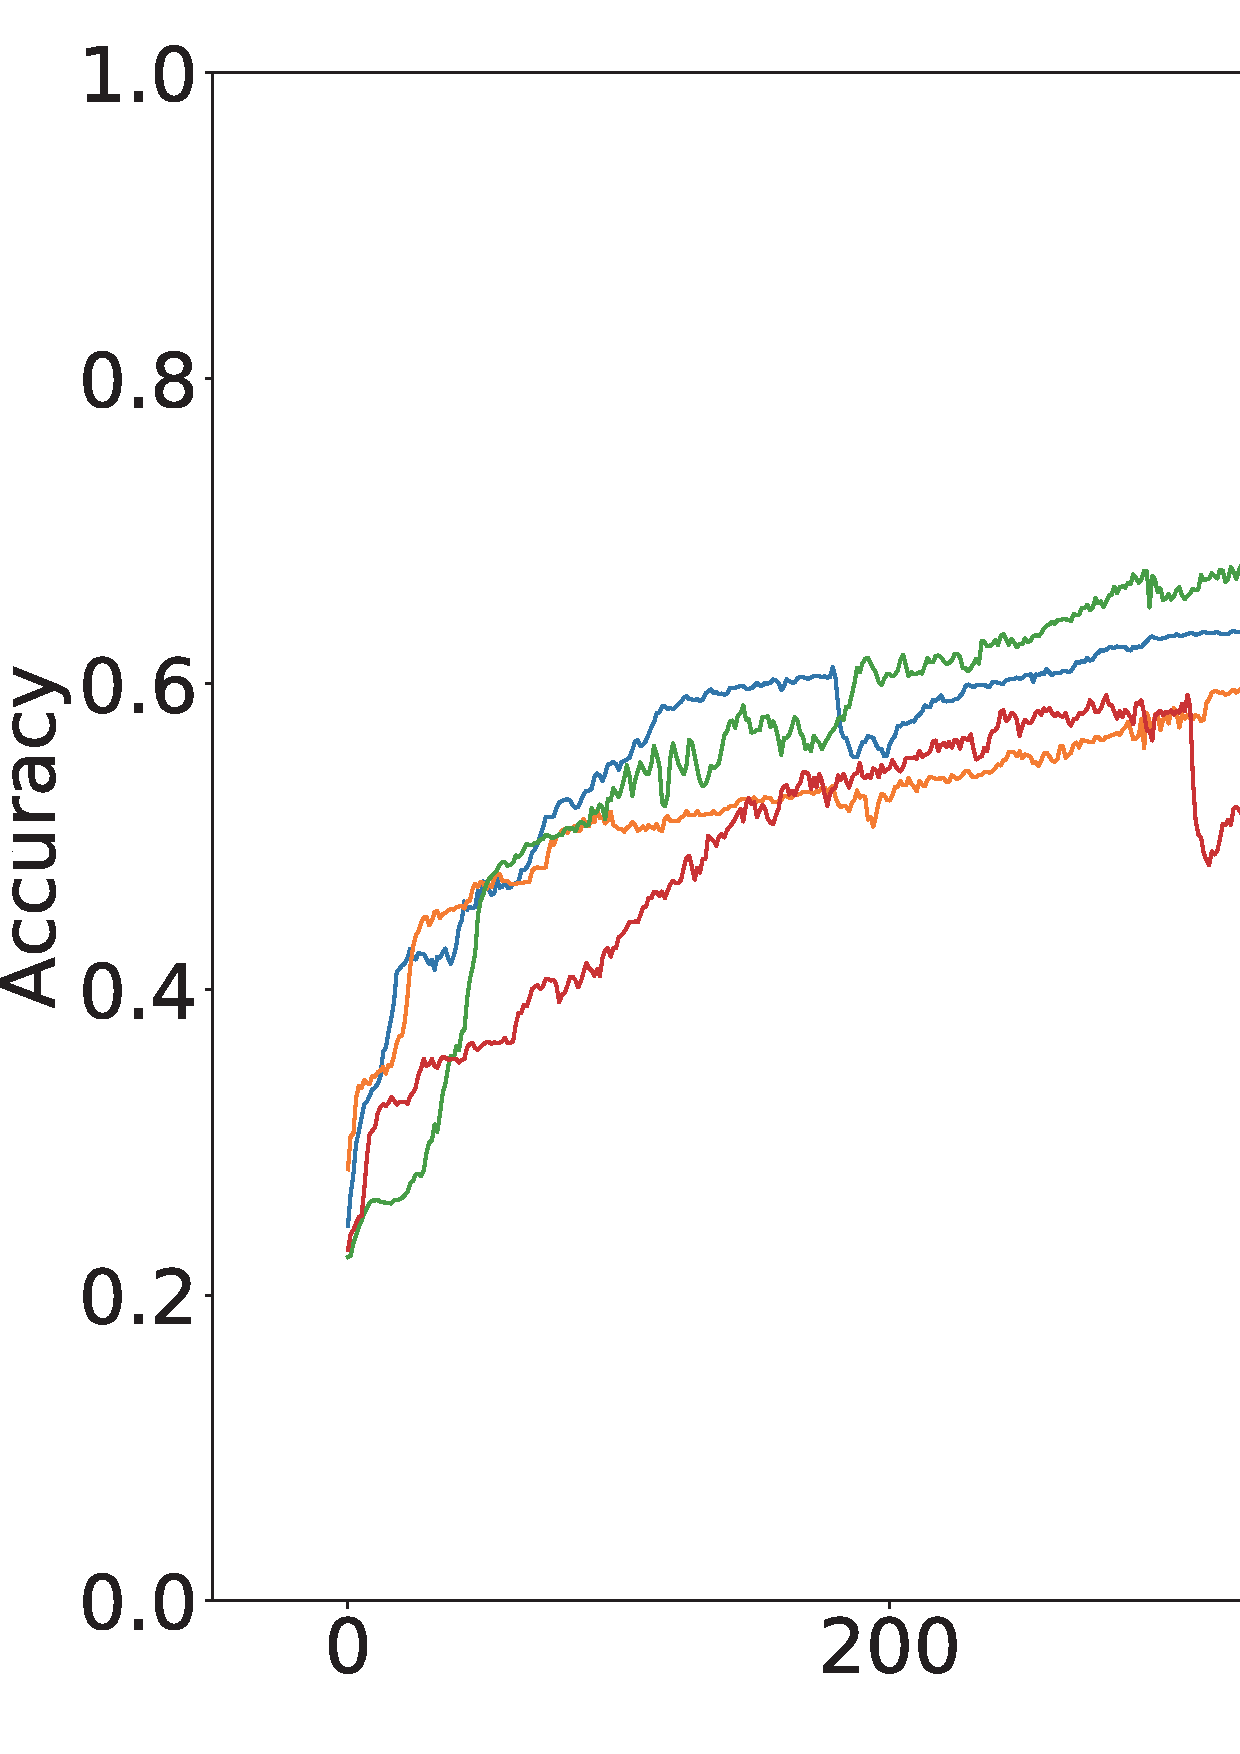
\includegraphics[width=0.75\linewidth]{Accuracy_micro}
% \caption{Accuracy of micro activities for training data (subject 1, 2, 3).}
% \label{fig:acc}
% \end{figure}

% \begin{figure}[h]
% \sidecaption[t]
% 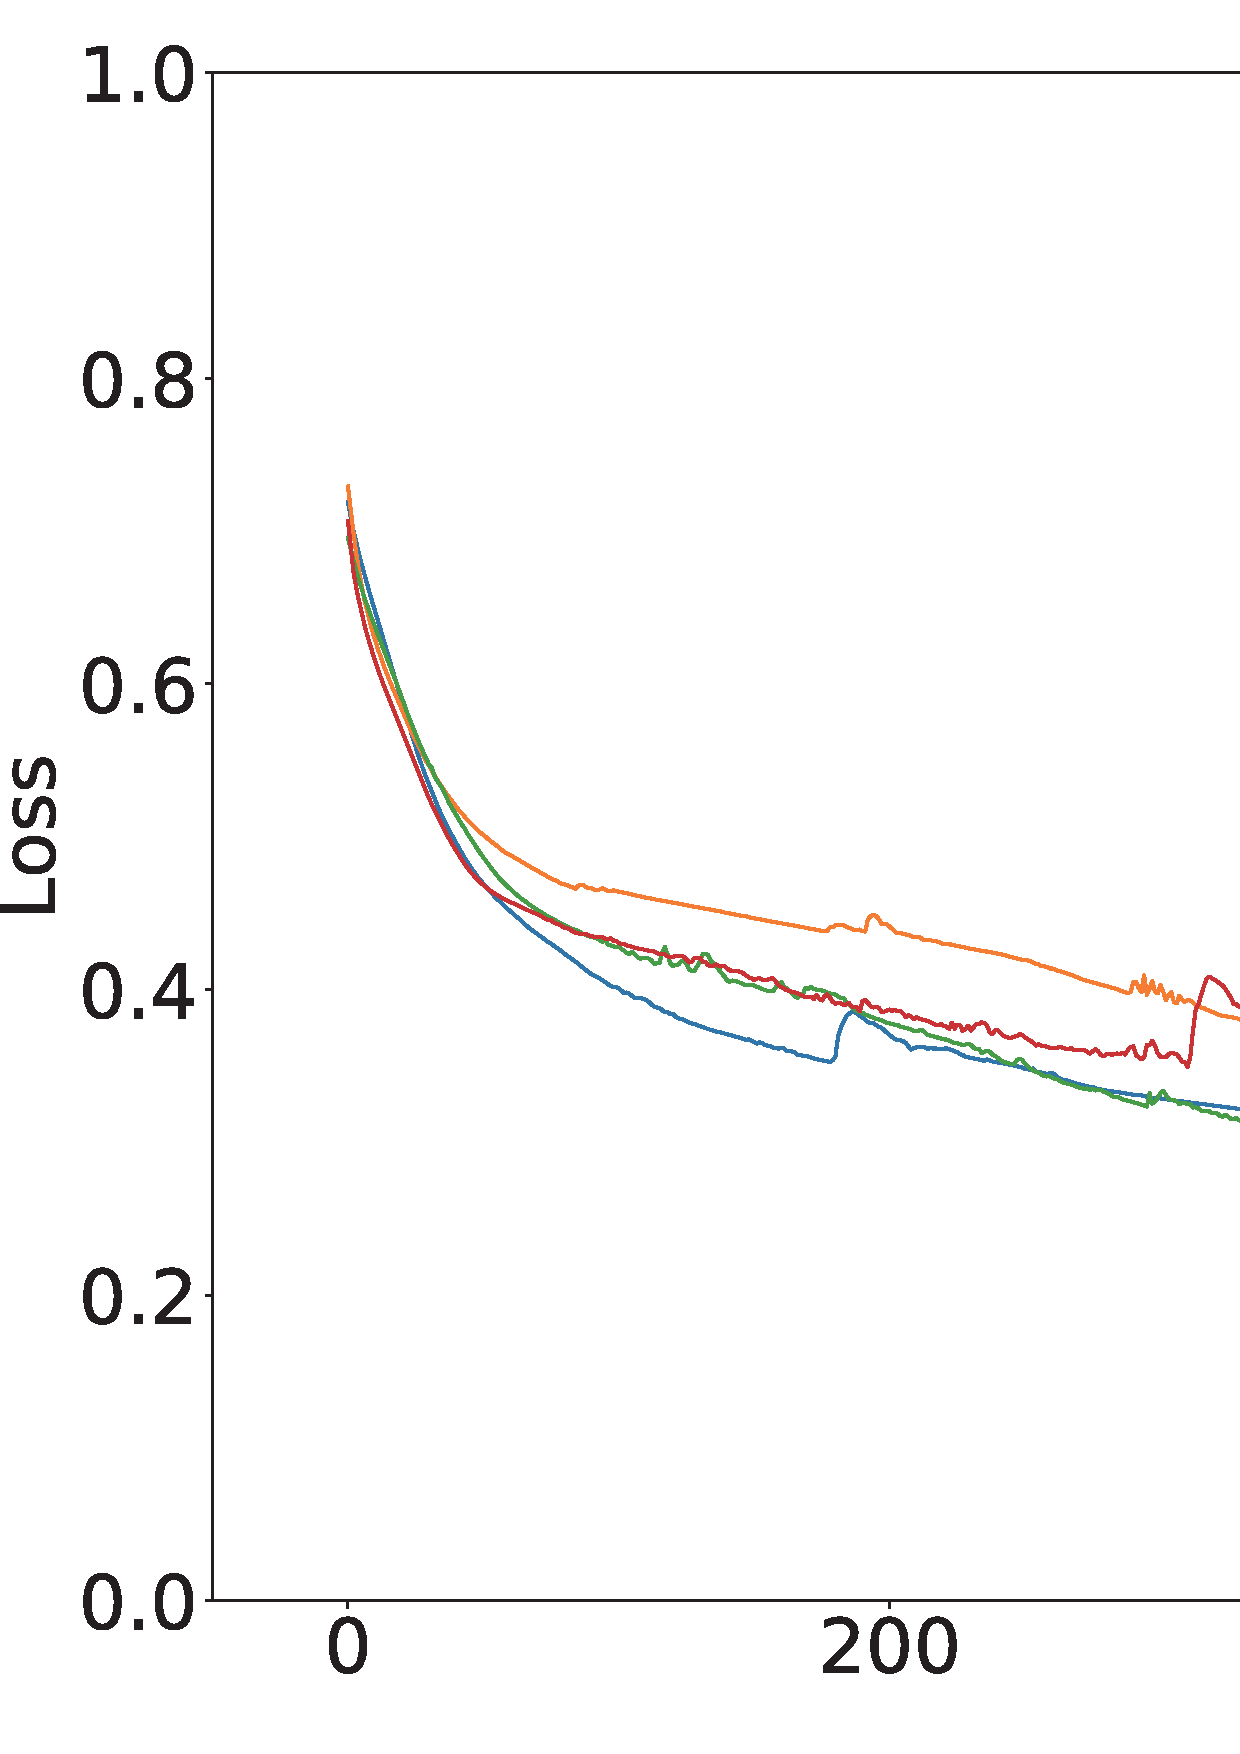
\includegraphics[width=0.75\linewidth]{Loss_micro}
% \caption{Loss of micro activities for training data (subject 1, 2, 3).}
% \label{fig:loss}
% \end{figure}

% \begin{figure}[h]
% \sidecaption[t]
% 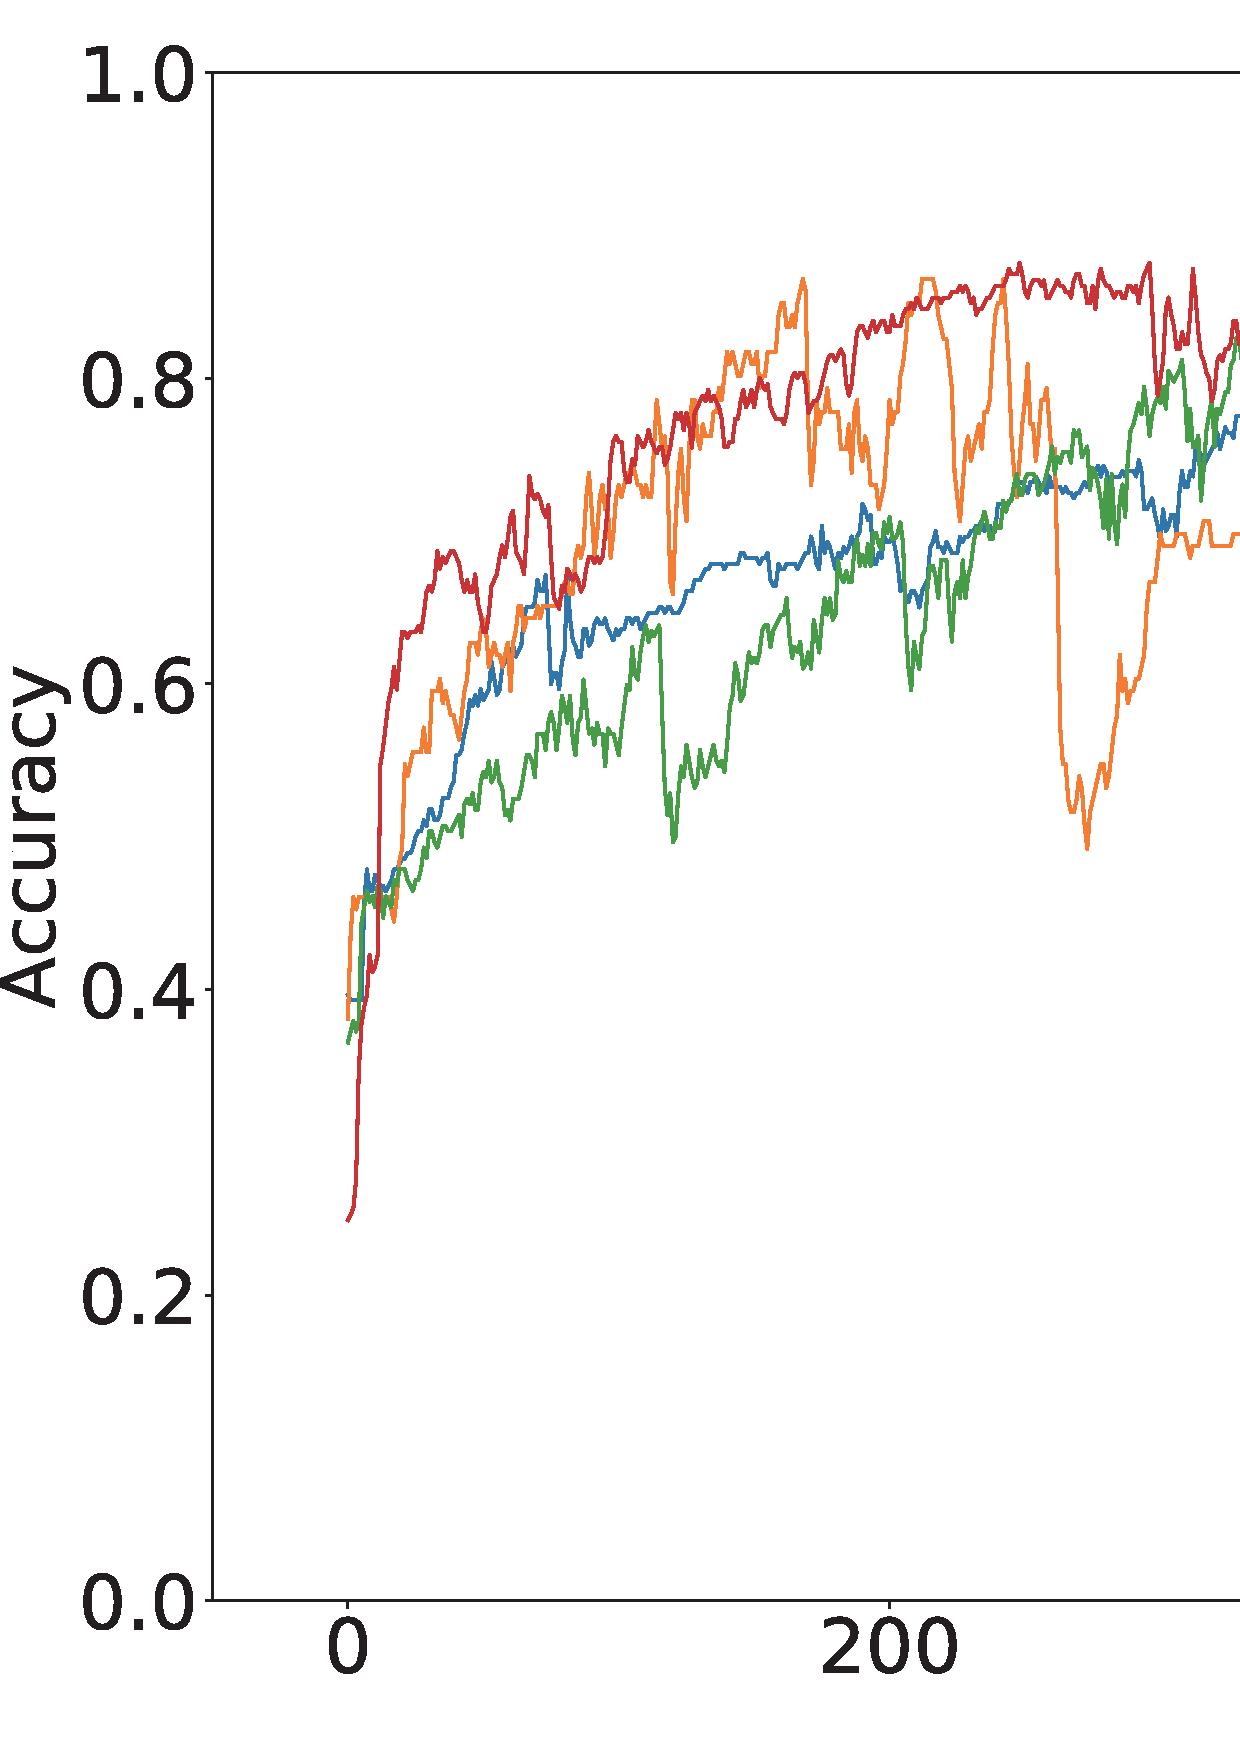
\includegraphics[width=0.75\linewidth]{Accuracy_macro}
% \caption{Accuracy of macro activities for training data (subject 1, 2, 3).}
% \label{fig:acc_recipe}
% \end{figure}

% \begin{figure}[h]
% \sidecaption[t]
% 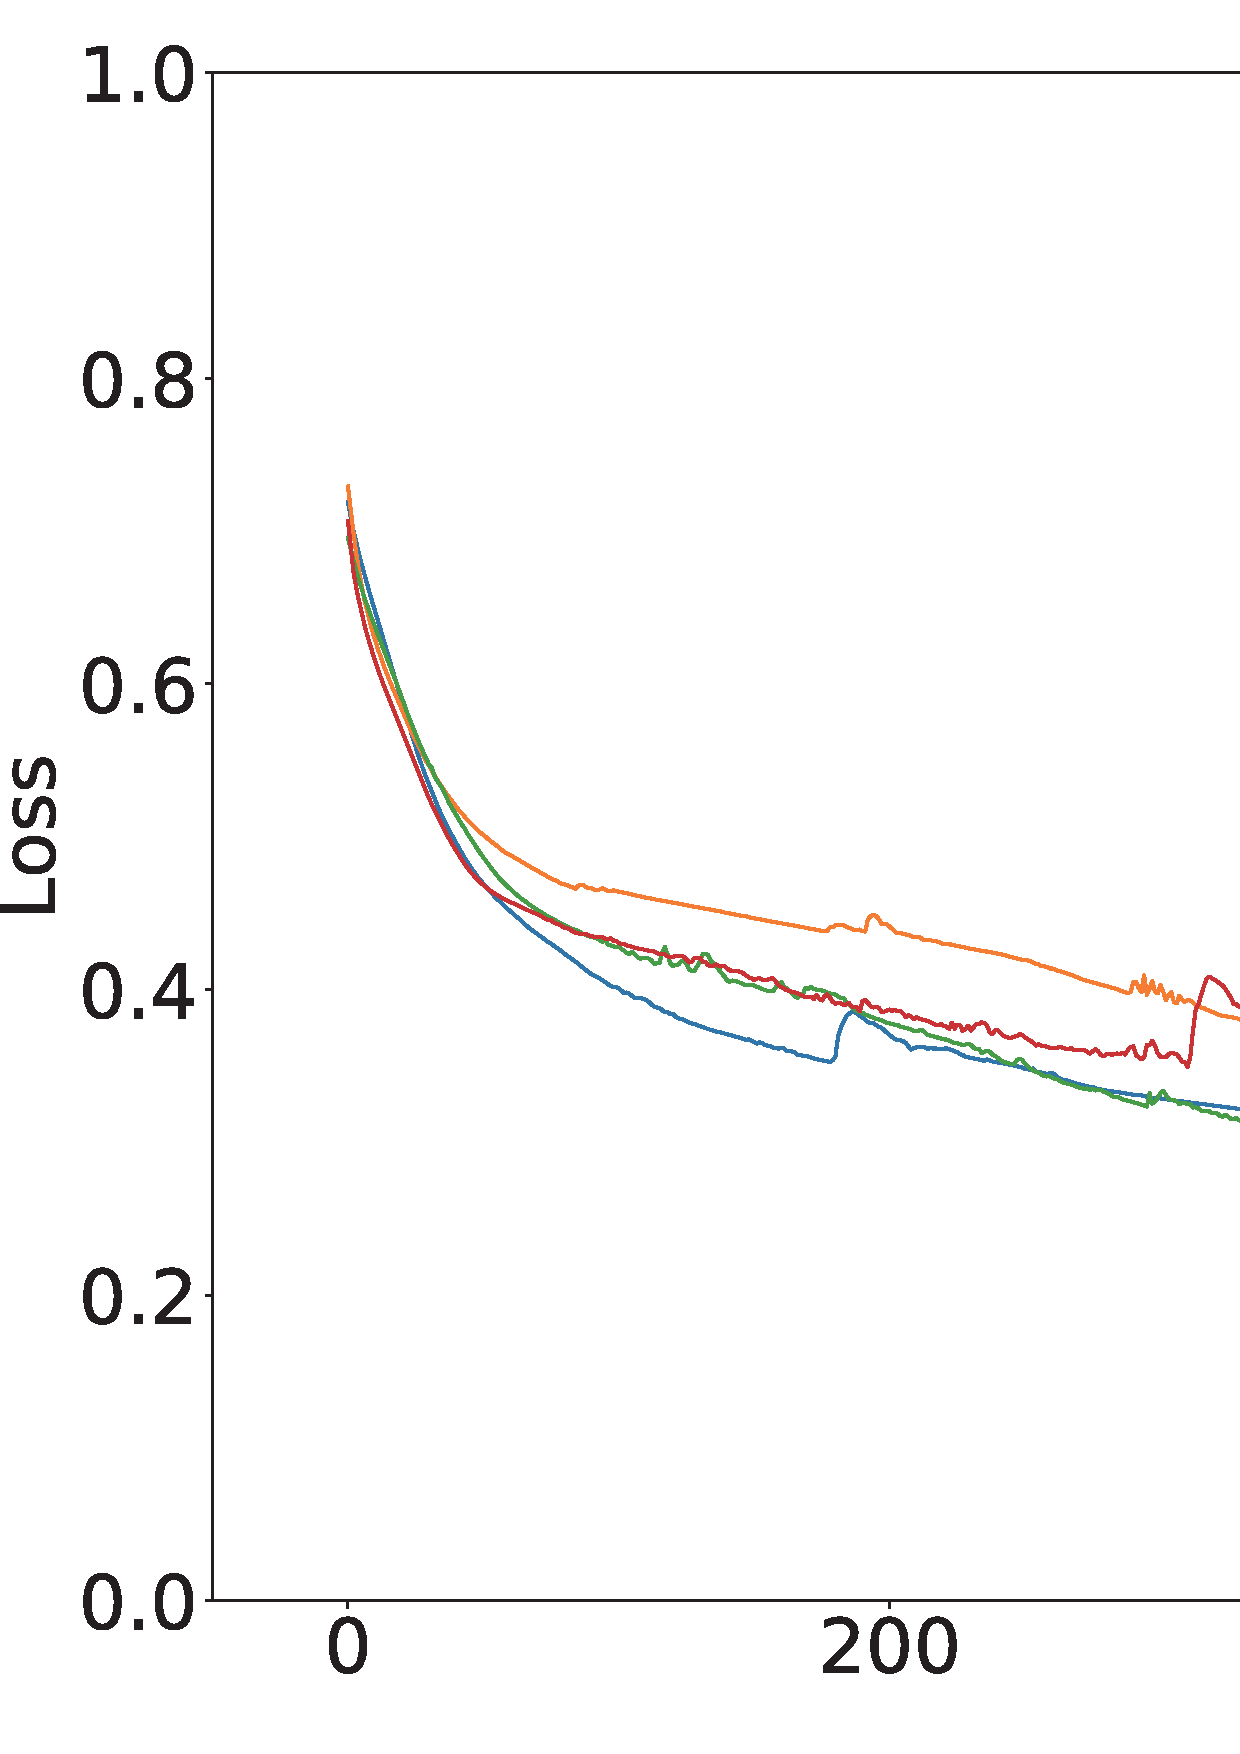
\includegraphics[width=0.75\linewidth]{Loss_micro}
% \caption{Loss of macro activities for training data (subject 1, 2, 3).}
% \label{fig:loss_recipe}
% \end{figure}

From these results, average accuracy of 0.522 and 0.491 were achieved among subjects 1, 2, and 3 for micro and macro activities, respectively. Considering ten multi-label micro activities, it would be said that 0.522 accuracy is good, while 0.491 accuracy for macro activity can be improved. For the result of training and testing data of subjects 1, 2, and 3, accuracy was improved as training data and testing data are same. Macro activity was better since the number of classes is three and the classes are not overlapping.

Note that for submitted result for the data of subject 4, our model was trained separately for the body parts with the data of subjects 1, 2, and 3, and the model at 1,000th epoch was used for testing the data of subject 4.

Table \ref{tab:resources} shows memory usage on CPU and GPU, and processing time taken in training phase and testing phase.

\begin{table}[!h]
    \caption{CPU and GPU memory usage and time taken in training and testing. These figures are when data of four body parts are processed at once.}
    \centering
    \begin{tabular}{c|c|c}\hline\hline
         Resource& Macro & Micro  \\\hline
         CPU memory& 2391MB &2391MB\\
         GPU memory& 1.6GB& 1.6GB\\
         Training time (1,000 epoch)& 21.554s & 28.891s \\
         Testing time (1,000 epoch)& 58.042s & 59.299s \\\hline
    \end{tabular}
    \label{tab:resources}
\end{table}


\section{Conclusion}
\label{sec:conclusion}
This paper reported the solution of our team ``Rits's cooking'' to Cooking Activity Recognition Challenge held at International Conference on Activity and Behavior Computing (ABC2020).

We plan to construct the streamline model without handcrafted features and majority vote.

\bibliographystyle{spmpsci}
\bibliography{bib}

\section*{Appendix}
\addcontentsline{toc}{section}{Appendix}
\subsection*{Used sensor modalities}
Four acceleration sensors at lest hip, left wrist, right arm, and right wrist from three subjects were used. Mocap data was NOT used.

\subsection*{Features used}
Seven kinds of features were used: Mean, variance, max, min, root mean square (RMS), interquartile range (IQR), and zero crossing rate (ZCR).
These features are extracted for x, y, and z axis, respectively.

\subsection*{Programming language and libraries used}
Python 3.6.7 was used. For network implementation, PyTorch 1.4.0 was used.

\subsection*{Window size and post processing}
Window size is 500 ms and step size is one sample.

\subsection*{Training and testing time}
Training time (1,000 epoch) was 21.554s for macro activity and 28.891s for micro activity.
Testing time (1,000 epoch) was 58.042s for macro activity and 59.299s for micro activity.

\subsection*{Machine specification}
OS: Windows 10 Pro. CPU: Intel Core i7-8700K 3.7KHz. RAM: DDR4 64GB. GPU: NVIDIA GeForce RTX 2080Ti GDDR6 11GB.

%




\end{document}
